\begin{frame}

\frametitle{Volumes and Partitions}

\begin{center}

A physical drive is perhaps partitioned into multiple volumes.

\end{center}

\vspace{\fill}

\begin{center}

A volume is a storage entity holding a filesystem.

\end{center}

\end{frame}


\begin{frame}

\frametitle{Mounting}

\begin{center}

\large \textbf{Unified filesystem}

\end{center}

\begin{itemize}

\item Start at \texttt{/}.

\item Mount any device anywhere.

\item Typical of UNIX, Linux, BSD.

\end{itemize}

\vspace{\fill}

\begin{center}

\large \textbf{Volume-first}

\end{center}

\begin{itemize}

\item All pathnames begin with a volumename.

\item Typical of Windows, KUDOS.

\end{itemize}

\end{frame}


\begin{frame}

\begin{center}

\Large \textbf{Cool, so can I put a volume in a file?}

\end{center}

\pause

\begin{flushright}

--- Of course, you can!

\end{flushright}

Some popular examples:

\begin{itemize}

\item ISO 9660, known colloquially as ``\texttt{.iso}-files''.

\begin{itemize}

\item The file-format we use to store copies of CDs.

\end{itemize}

\item \texttt{squashfs}, a compressed, read-only filesystem.

\begin{itemize}

\item Used in a Linux live-CD near you.

\end{itemize}

\item TFS in your KUDOS.

\end{itemize}

\end{frame}


\begin{frame}

\begin{center}

\Huge \textbf{DEMO}

\bigskip

\large The \texttt{dd} and \texttt{mkdosfs} utilities\ldots and \texttt{mount}.

\end{center}

% dd if=/dev/zero of=fatdisk bs=1M count=64
% mkdosfs -F 32 fatdisk

\end{frame}


\begin{frame}[fragile]

\frametitle{DEMO: Log (1/3)}

\begin{itemize}

\item Create something that looks like a disk:

\begin{verbatim}
$ dd if=/dev/zero of=fatdisk bs=1M count=64
64+0 records in
64+0 records out
67108864 bytes (67 MB, 64 MiB) ...
\end{verbatim}

\item Turn \texttt{fatdisk} into a FAT32 volume (\textbf{format} as FAT32):

\begin{verbatim}
$ mkdosfs -F 32 fatdisk
mkfs.fat 3.0.28 (2015-05-16)
\end{verbatim}

\item Check your work:

\begin{verbatim}
$ file fatdisk 
fatdisk: DOS/MBR boot sector...
OEM-ID "mkfs.fat"... FAT (32 bit) ...
\end{verbatim}

\item OEM-ID might tell you who formatted the volume.

\end{itemize}

\end{frame}


\begin{frame}[fragile]

\frametitle{DEMO: Log (2/3)}

\begin{itemize}

\item Mount that "disk":

\begin{verbatim}
$ ... mount fatdisk workdir -o rw,umask=0000
\end{verbatim}

\item Copy our file to it, and unmount:

\begin{verbatim}
$ cp foo workdir/
$ ... umount workdir/
\end{verbatim}

\item Now let's write it to disk!

\begin{verbatim}
$ ... dd if=fatdisk of=/dev/sdb1
\end{verbatim}

\item \texttt{/dev/sdb1} is a partition on my USB drive, use \texttt{... fdisk
-l} to find such partitions.

\begin{verbatim}
$ ... fdisk -l
...
/dev/sdb1        ...  3.8G  b W95 FAT32
\end{verbatim}

\end{itemize}

\end{frame}


\begin{frame}[fragile]

\frametitle{DEMO: Log (3/3)}

\begin{itemize}

\item Check your work:

\begin{verbatim}
$ ... mount /dev/sdb1 workdir/
$ cat workdir/foo
hello
$ umount workdir/
\end{verbatim}

\end{itemize}

\end{frame}


\begin{frame}

\begin{center}

\Large \textbf{Cool, so should I try this at home?}

\end{center}

\begin{flushright}

--- Yes, but beware\ldots

\end{flushright}

\begin{itemize}

\item It is easy to \texttt{sudo dd if=... of=/dev/sda}

\item \texttt{/dev/sda} is typically your main harddrive.

\item Linux \textbf{will not} stop you.

\item Mount the device directly, don't \texttt{dd} filesystems (too often).

\item As on the previous slide.

\end{itemize}

\end{frame}


\begin{frame}

\frametitle{DEMO: Screenshots (1/2)}

\begin{center}

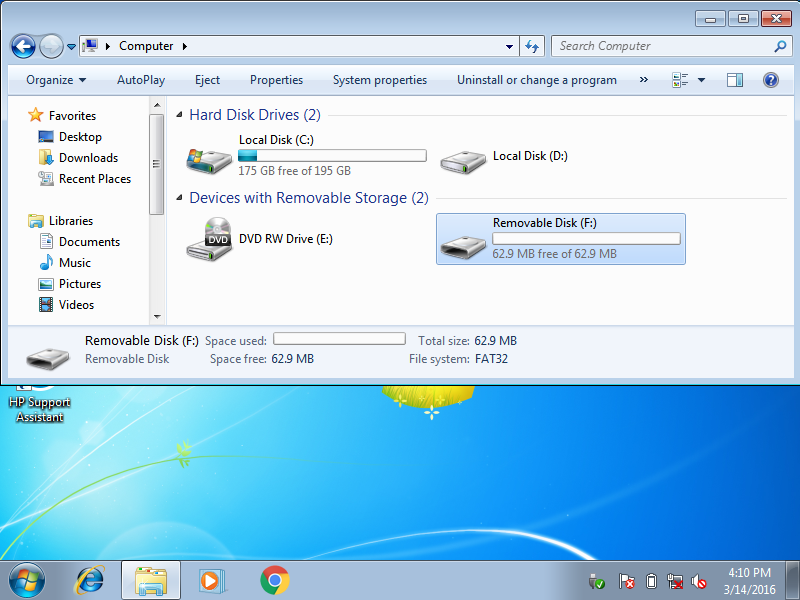
\includegraphics[scale=0.4]{figures/windows-mycomputer}

\end{center}

\end{frame}


\begin{frame}

\frametitle{DEMO: Screenshots (2/2)}

\begin{center}

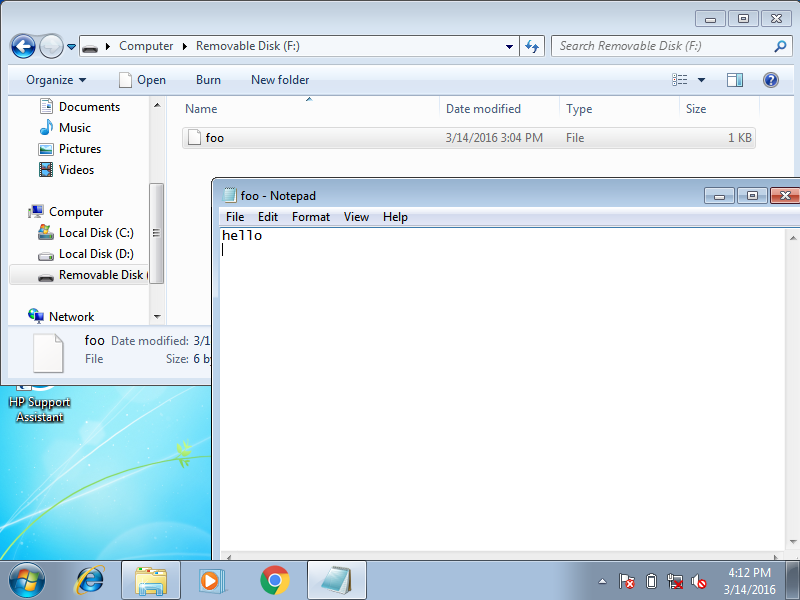
\includegraphics[scale=0.4]{figures/windows-foo}

\end{center}

\end{frame}
